%!TEX  root = main.tex
\chapter{Délimitation de l'objet d'étude}
\label{ch:methodo}

\PartialToc


Une démarche de recherche classique commence par la formulation d'une question 
de départ. La question qui a initié nos travaux est la suivante~: «~comment 
simuler, afin de les valider, les SI des Smart Grids?~».  Comme en témoigne notre 
état de l'art, cette question fait l'objet de très peu de travaux (section 
\ref{approche_simu_existante}). Une phase exploratoire préalable a donc été nécessaire 
pour mettre en évidence les caractéristiques de notre objet d'étude. À cet effet,
une démarche de recherche inductive a été jugée pertinente.

Nous exposons cette démarche en la justifiant dans la section~\ref{sec:demarche_objet_etude}.
Puis, nous reprenons les étapes de cette phase exploratoire 
par ordre chronologique~: exploration de la vue métier dans la section~\ref{sec:exploration_metier}, puis celle de la vue 
applicative dans la section~\ref{sec:investig_appli} et en fin celle de la vue fonctionnelle dans 
la section~\ref{sec:exploration_fonctionnelle}.
Cependant, nous ne cherchons pas à donner l'impression que notre plan de recherche a été 
entièrement établi avant de le mettre en œuvre. Au contraire, nous l'avons 
construit au fur et à mesure de nos interactions avec le terrain d'étude. 

% expliquer ce que c'est une approche inductive.

% Cette phase exploratoire a été préalable et indipensable à la définition du cadre d'architecture 
% \textit{ExcuteEA}. 


% L'intérêt de cette partie est de traiter la question de la cohérence entre nos 
% objectifs de recherche et la démarche que nous adoptons pour y répondre. 




\section{Démarche engagée}
\label{sec:demarche_objet_etude}
		
Dans ces travaux de thèse, une attention particulière est apportée à la délimitation de l'objet d'étude. 
Cette délimitation est souvent le résultat de l'observation du terrain d'étude~: 
l'entreprise et son SI d'une manière générale et l'entreprise et son SI dans le 
cas particulier des Smart Grids. L'entreprise et son SI forment un système 
complexe dont l'observation n'est pas triviale. La délimitation de l'objet 
d'étude a donc été, en soi, à l'origine d'une démarche de recherche.

Nous avons adopté pour cela une démarche de recherche inductive et ce pour plusieurs raisons.
D'une part, une démarche inductive est pertinente pour formuler des hypothèses ou soulever des questions,
et pour aborder un sujet qui a été peu étudié comme c'est le cas de la simulation du SI des Smart Grids.	
Cette démarche est donc adaptée pour~: 
\begin{enumerate}
	\item délimiter l'objet de l'étude, c'est à dire identifier ce qui est dans le 
contexte de la simulation des SI et ce qui ne l'est pas~;
	\item jeter les bases d'une étude théorique ultérieure.
\end{enumerate}
	
D'autre part, l'induction est une démarche de recherche classique en sciences 
sociales. Elle correspond au raisonnement empiriste qui affirme que 
l'observation et l'expérience sont la source de la connaissance du monde réel et 
du concret \cite{madeleine2001methodes}. Nous cherchons en effet à comprendre 
notre objet d'étude empiriquement. Le recours à cette démarche est d'autant plus 
justifié par la nature socio-technique du SI. En définissant le SI, Robert Reix 
met en évidence sa composante sociale (voir chapitre \ref{ch:EA}). 
	
%Une étude ethnographique est Notre démarche inductive est donc doublée d'.

La volonté de délimitation de notre objet d'étude est portée par la question 
suivante «~Qu'est-ce que la simulation d'un SI d'entreprise ?~». Néanmoins, même 
empirique, une démarche de recherche doit nécessairement s'inscrire dans un 
cadre de cohérence. Nous avons donc veillé à construire un protocole 
d'investigation épistémologiquement valide et conforme aux critères de cohérence 
interne. Notre protocole d'investigation est axé sur l'observation et 
l'expérience. Il est constitué de trois grandes étapes ~:
		
\begin{enumerate}
	\item observation du terrain d'étude, c'est à dire analyse des pratiques 
courantes des personnes impliquées par la simulation des SI des Smart Grids. Nous avons identifié deux 
catégories de personnes susceptibles d'être concernées~: les personnes appartenant au domaine du SI (ou 
de sa simulation), et les personnes susceptibles d'instrumenter la simulation des SI 
pour leurs travaux de recherche ou d'ingénierie (il s'agit là des utilisateurs 
finaux). Nous avons privilégié les ingénieurs-chercheurs d'\gls{edf}~R\&D car le 
contexte \gls{cifre} de la thèse a facilité l'accès à ces 
personnes. L'observation aboutit à la formulation d'hypothèses «~aprioristes~». 
Ce sont des hypothèses exploratoires visant à soulever des interrogations~;

	%observation participative, démarche ethnographique
	
	\item développement d'un prototype de simulation tenant compte du résultat des 
observations de l'étape précédente. Le prototype n'a pas pour vocation de 
proposer une solution finale mais plutôt de tester rapidement les hypothèses 
formulées précédemment~;
	
	\item validation ou mise à l'épreuve du prototype sur le terrain d'étude. Cette 
mise à l'épreuve commence par la définition d'un cas d'application pertinent 
permettant de vérifier les hypothèses formulées à l'étape d'observation. Elle se 
poursuit par la collecte et l'analyse du retour des personnes concernées. Le 
contexte \gls{cifre} a là aussi facilité les échanges avec les 
ingénieurs-chercheurs de EDF R\&D, et en particulier ceux du département 
\gls{mire}. Notre intégration à l'équipe des ingénieurs-chercheurs du département 
\gls{mire}, et en particulier à l'équipe du projet de simulation des Smart Grid, 
a contribué à la qualité des échanges avec les personnes interrogées.
	
\end{enumerate}
		
Le raisonnement par induction aboutit à des propositions générales à partir de 
cas singuliers. Nous avons donc commencé par décomposer le terrain d'étude, 
c'est à dire le SI de l'entreprise. Les bases théoriques de la discipline des SI 
ont permis de procéder à cette décomposition afin de mettre en évidence ses 
singularités. Les approches par points de vue sont largement utilisée pour 
traiter la complexité des SI en le décomposant en plusieurs vues~: la vue 
métier, la vue fonctionnelle, la vue applicative, la vue technique. Chaque vue 
correspond à la perspective d'un groupe de personnes aux profils différents mais 
complémentaires. Les investigations ont été menées sur les trois premières vues — 
métier, fonctionnelle, applicative. La vue technique n'a pas été traitée~: le 
temps nécessaire aux expérimentations est incompatible avec les délais de cette 
thèse et son financement dans le cadre d'une \gls{cifre}.
	
Le protocole d'investigation est alors appliqué à chacune des vues métier, 
fonctionnelle et applicative. L'objectif de la démarche engagée est de définir 
l'objet d'étude, en ayant comme question de départ «~Qu'est-ce que la simulation 
d'un SI d'entreprise ?~». Cependant, nous avons veillé à garder une capacité 
d'ouverture aux idées nouvelles. %Nous présentons
	
\section{Investigations menées pour la vue métier}
\label{sec:exploration_metier}
La première étape d'observation a débuté avec un stage de fin d'étude de six 
mois que nous avons effectué au sein du département \gls{mire}. L'objectif du 
stage a consisté à explorer le sujet «~Simulation du SI des Smart Grids~» afin 
de préparer un sujet de thèse. Il s'est donc accordé avec l'objectif des 
investigations menées pour la vue métier.
			
\subsection{Observation}
Pour cette première phase d'observation, des entretiens ont été menés avec 
des experts SI internes à l'entreprise, mais aussi externes à celle-ci lors 
d'un séminaire professionnel ayant pour thème la modélisation des SI \footnote{Model Driven Day, 21 novembre 2001, Paris 
Cœur Défense}. Des entretiens ont aussi été menés avec des ingénieurs-chercheurs 
du département \gls{mire} ayant participé à des démonstrateurs Smart Grids 
européens pour mettre en évidence les pratiques de spécification de la 
composante SI des Smart Grids. 

Les hypothèses formulées à l'issue des ces observations sont les suivantes~:
\begin{itemize}
    \item la simulation de SI est une discipline peu étudiée~;
	\item la simulation des processus métier est pertinente pour les SI des 
Smart Grids dans la mesure ou elle permet de valider les scénarios élaborés pour 
les démonstrateurs, mais aussi pour les SI tout court~;
	\item lors de cette simulation, il est nécessaire de maintenir une 
cohérence entre le processus et les données qu'il manipule~;
	%\item les langages de modélisation exécutables présentent des avantages pour la simulation des SI.
\end{itemize}
		
\subsection{Prototypage}
Le prototypage a nécessité une étude des outils existants proposant de 
simuler des processus métier, ce qui a permis d'identifier les outils suivants~: 
Enterprise Architect, Bonita, Amuse et Rhapsody. Il a ensuite fallu évaluer leur capacité de simulation selon une grille d'évaluation. Le critère de 
sélection principal a été la capacité de l'outil à exécuter des diagrammes 
d'activité UML. En effet, c'est dans ce langage que sont représentés les 
processus métier dans les documents de spécification des démonstrateurs Smart 
Grid. Le deuxième critère d'évaluation retenu a été la possibilité d'ajout de 
nouvelles fonctionnalités à l'outil. À l'issue de cette étude comparative, 
l'outil Enterprise Architect dans sa version 9.2 a été retenu. En effet, à 
l'époque de l'étude, EA était le seul à pouvoir animer des diagrammes d'activité 
et à offrir la possibilité d'ajout de fonctionnalité par le mécanisme de plugin. 
C'était en outre l'outil de modélisation UML de référence de l'équipe 
d'ingénieurs-chercheurs au sein de laquelle nous avons effectué ce stage.
				
Cependant, dans sa version 9.2, l'outil n'assure pas la cohérence entre les 
objets métier (modélisés avec des diagrammes de classes) et le processus (modélisé 
avec un diagramme d'activité) au cours de la simulation. De plus, l'outil ne 
gère pas la persistance des résultats de la simulation. La mise en cohérence a 
donc nécessité le développement d'un plugin que nous avons baptisé DataSimu. 
DataSimu permet de (1)~créer un jeu de données en entrée de la simulation à 
partir des concepts métier en instanciant un diagramme de classes (2)~simuler le 
processus métier avec ce jeu de données (3)~récupérer le jeu de données en sortie 
de la simulation et le stocker dans une base de données. Nous avons mené 
l'implémentation de DataSimu en binôme avec un étudiant en troisième année 
d'école d'ingénieur. L'interface graphique de DataSimu est illustrée par la 
figure~\ref{fig:data_simu}.
%L'annexe~\ref{annexe:datasimu} détaille l'architecture de DataSimu et présente un 
%manuel d'utilisation. 
				
\begin{figure}[!ht]
  \centering
  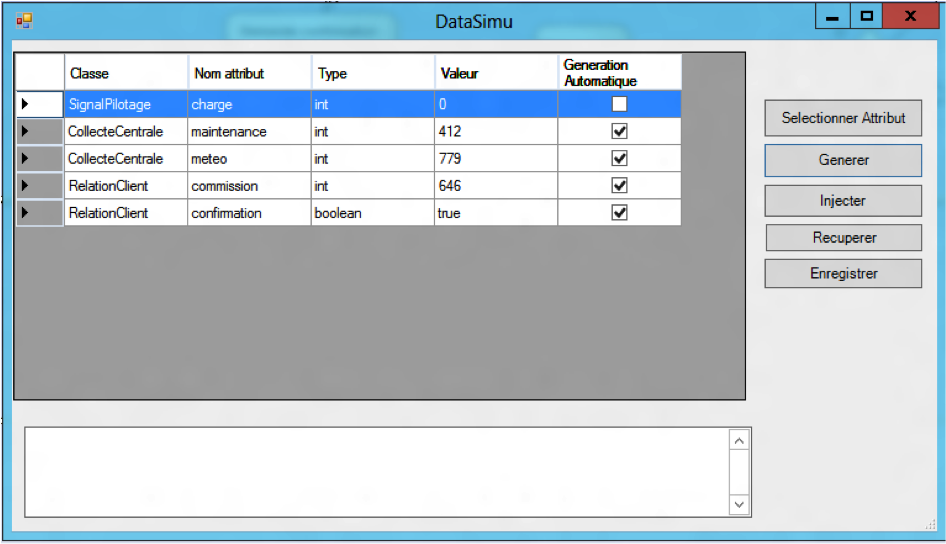
\includegraphics[width=1\textwidth]{figures/6_methodologie/data_simu.png}
  \caption{Interface Graphique de DataSimu}
  \label{fig:data_simu}
\end{figure}
				
\subsection{Validation}
Pour valider les hypothèses formulées à l'issue de l'observation, un cas 
d'application Smart Grid a été mis au point~: le pilotage d'une charge 
domestique. Ce cas d'application est issu de l'étude des spécifications des 
démonstrateurs Smart Grid ADDRESS et PREMIO introduits dans la 
section~\ref{sec:DemonstrateursSG}. Il s'agit de piloter une batterie de 
stockage d'énergie installée chez un client (particulier ou industriel). En 
fonction de l'état du réseau, une centrale de pilotage contrôle cette batterie 
(stockage d'énergie pour une utilisation ultérieure), tout en tenant compte des 
consignes du client. Ce cas métier a été modélisé et simulé avec l'outil 
Enterprise Architect doté du plugin DataSimu.
%Une description détaillée du cas 
%métier et du déroulement de la simulation est donnée dans l'annexe~\ref{annexe:datasimu}.
			
Le prototype de simulation et sa mise en œuvre à travers le cas métier du 
pilotage d'une charge domestique ont été soumis aux experts SI du département 
\gls{mire} et aux ingénieurs-chercheurs contribuant aux démonstrateurs Smart 
Grid PREMIO et ADDRESS. Les entretiens suivant la démonstration ont validé (1) 
la pertinence de la simulation dans le contexte des SI des Smart Grids (2) la 
séparation du processus métier et des objets métier tout en maintenant une 
cohérence lors de la simulation.
			
Ces entretiens, assortis à l'étude des outils de simulation des processus 
métier, ont permis de constater que la question de la simulation est peu abordée 
dans le contexte des SI. Ces travaux d'investigation ont de plus donné lieu à 
une publication \cite{seghiri2012animation} et ont été poursuivis par les 
travaux présentés dans cette thèse.
 
\subsection{Conclusion}
Cette première application du protocole d'investigation a conforté nos hypothèses initiales à savoir que la simulation est peu abordée dans le contexte des SI mais qu'elle est pertinente pour valider/critiquer les scénarios de cas métier Smart Grid avant leur implémentation.

\section{Investigations menées pour la vue applicative} 
\label{sec:investig_appli}
La vue applicative tient une place de choix dans les SI des entreprises. Pour des SI fortement informatisés, il arrive même souvent que le SI soit réduit aux applications informatiques et à l'infrastructure qui les supporte. Cette constatation est encore plus avérée dans le cas des Smart Grids dont le principe est le déploiement de TIC sur le réseau électrique pour automatiser son pilotage. Le choix chronologique de poursuivre les investigations en abordant la vue métier découle de cette constatation.		
			
\subsection{Observation}
Les investigations menées pour la vue applicative ont nécessité d'approfondir nos connaissances du fonctionnement du réseau électrique. Pour cette deuxième phase d'observation, nous avons conduit des entretiens avec deux profils de personnes~: des experts et des ingénieurs-chercheurs spécialisés dans le réseau électrique de distribution  appartement au département \gls{mire}. En effet, plus que les réseaux de transport, ce sont les réseaux de distribution qui sont concernés par les Smart Grids. Les réseaux de transports français sont déjà fortement automatisés. 
L'objectif de ces entretiens est double~: approfondir nos connaissances du réseau électrique et comprendre les pratiques des personnes interrogées en matière de simulation.
Les experts sus-mentionnés sont responsables de la conception d'applications pour la conduite du réseau électrique. Le langage de conception le plus utilisé est les automates programmables. Les ingénieurs-chercheurs sont quand à eux responsables du développement des applications, le plus souvent en Matlab ou C++.
Les hypothèses formulées à l'issue de cette observation sont les suivantes~:
\begin{itemize}
    \item la simulation du SI pour les Smart Grid est liée à la simulation des réseaux électriques~;
	\item la simulation du SI des Smart Grid nécessite de traiter la problématique de l'hétérogénéité des modèles.
\end{itemize}
				
\subsection{Prototypage}
				
Nous avons utilisé l'outil de modélisation hétérogène Ptolemy\footnote{http://ptolemy.eecs.berkeley.edu/} pour développer un prototype de simulation illustré par la figure~\ref{fig:simu_ptolemy}. L'observation a permis d'identifier les éléments à modéliser, à savoir le SI et le réseau électrique. Ici l'hétérogénéité des modèles provient de leur dépendance au temps. La modélisation du comportement du SI et celle du réseau électrique font intervenir deux domaines de calcul différents~: à événements discrets pour le SI, et à flots de données périodiques pour le réseau électrique. 
Ainsi, dans le modèle Ptolemy illustré par la figure ~\ref{fig:simu_ptolemy}, le domaine de calcul adopté pour le SI est \textit{Discrete Events} (DE), celui adopté pour le réseau de distribution électrique est \textit{Synchronous Data Flow} (SDF). Ptolemy permet d'adapter ces deux domaines de calcul pendant la simulation d'un cas métier et d'adresser l'hétérogénéité des modèles du SI et du réseau électrique. 

\begin{figure}[!ht]
  \centering
  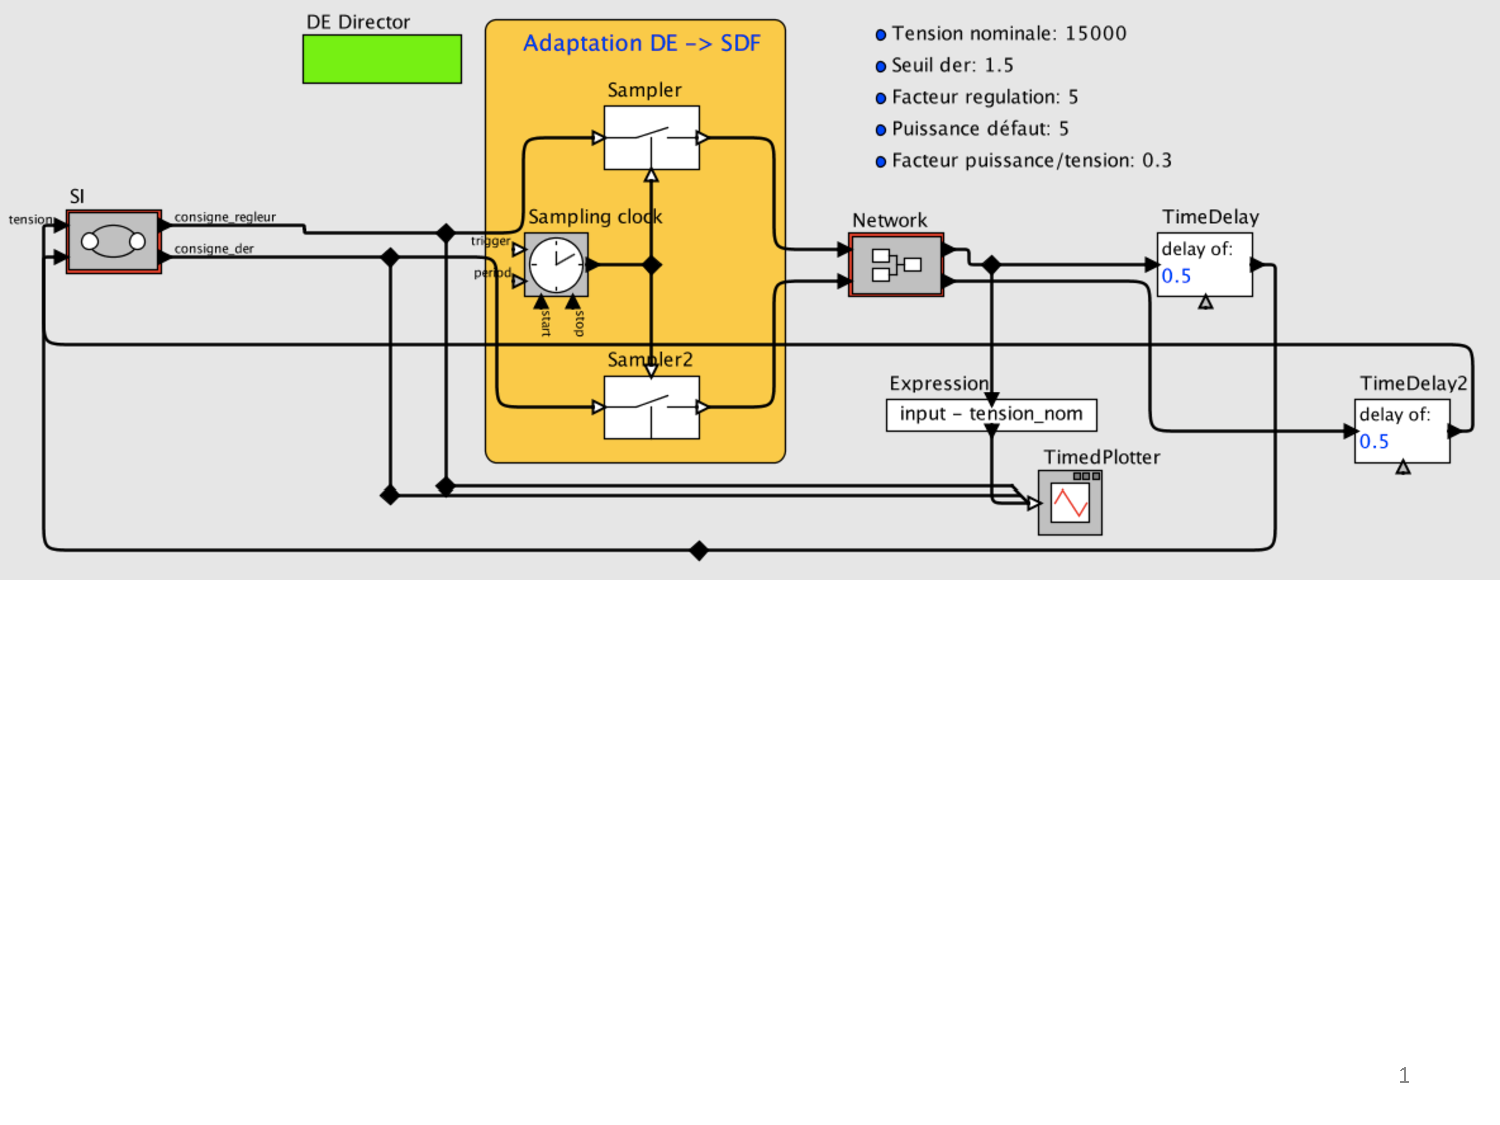
\includegraphics[trim = 0cm 8cm 0cm 0cm, clip, width=1\textwidth]{figures/6_methodologie/simu_ptolemy.pdf}
  \caption{Prototype Ptolemy pour une simulation hétérogène comprenant \\
           le SI (discret) et le réseau électrique (continu)}
 \label{fig:simu_ptolemy}
\end{figure}
		
\subsection{Validation}
Le cas d'application du pilotage d'une charge domestique n'a pas été utilisé pour le prototypage de la vue applicative. Les modèles de la vue applicative nécessitent un niveau de détail plus élevé que les modèles de la vue métier. Or les spécifications des démonstrateurs ADDRESS et PREMIO n'offrent pas le niveau de détail nécessaire. Le \textit{Use Case} normalisé par \gls{enel} (voir section~\ref{sec:ENEL}) pour la régulation de tension sur les réseaux de distribution a été adopté et affiné par les discutions avec les ingénieurs-chercheurs du département \gls{mire} travaillant sur la même thématique. 
		
Ils s'agit d'adapter la tension du réseau électrique en fonction de la charge et de la production pour maintenir un niveau de tension acceptable. Deux leviers d'action sont utilisés, les régleurs en charge et les \gls{der}. Les régleurs en charges pilotés à distance agissent sur le niveau de tension au niveau des postes sources. Le pilotage des \gls{der} permet de contrôler la quantité d'énergie qu'ils injectent sur le réseau. Ce cas métier fait intervenir un SI qui calcule les consignes envoyées aux DER et au régleur en charge, et un réseau électrique qui réagit à ces consignes. Il est à noter que le SI est réduit à sa vue purement applicative en ne de modélisant que l'application qui calcule les consignes.
		
		Ce cas métier a été modélisé puis simulé avec l'outil Ptolemy de modélisation et de simulation hétérogènes. Le comportement du SI est modélisé avec une machine à états qui calcule des consignes pour le DER et le régleur en charge en fonction du niveau de tension du réseau électrique. Le DER et le régleur en charge régulent la tension du réseau électrique en appliquant ces consignes. Le réseau de distribution est composé d'un DER, d'un consommateur d'électricité et d'un régleur en charge dont les comportements font varier le niveau de tension.
		
		La simulation de la régulation de tension avec Ptolemy a été soumise aux experts et ingénieurs chercheurs identifiés dans la phase d'observation. Bien que leurs retours aient permis de confirmer les hypothèses formulées concernant la problématique de l'hétérogénéité, cette problématique a été écartée de notre périmètre de recherche. En effet, les ingénieurs-chercheurs spécialistes du réseau électrique de distribution utilisent leur propres outils de simulation. Le prototype développé a permis de mettre en évidence la problématique de l'hétérogénéité des modèles mais pas de la résoudre. Un projet de co-simulation des domaines SI, réseau électrique et télécommunication a été lancé, suite aux résultats de différents projets de simulation dans le département \gls{mire}, dont nos travaux de thèse pour le domaine SI.


\subsection{Conclusion}
Cette deuxième application du protocole d'investigation pour la vue applicative a permis de confirmer nos hypothèses concernant la problématique de l'hétérogénéité des modèles de simulation mais surtout de réduire notre périmètre de recherche. En effet, l'hétérogénéité est traitée par un projet du département \gls{mire}, auquel nos travaux ont été intégrés. L'implémentation du cas métier de la régulation de tension à l'aide de Ptolemy, et le retour qu'en ont fait les personnes interrogées, nous a en outre permis d'affiner le cas métier de la régulation de tension. Sa réutilisation pour les investigations menées pour la vue fonctionnelle en a été d'autant plus facilitée.   

\section{Investigations menées pour la vue fonctionnelle} 
\label{sec:exploration_fonctionnelle}

La vue fonctionnelle est une vue charnière entre le métier et les applications qui  implémentent les processus métier. En effet, elle décompose chaque tâche métier en fonctions. Les investigations menées sur la vue fonctionnelle sont essentielles dans la mesure où cette vue permet de maintenir le lien entre le métier et l'IT. 

\subsection{Observation}
Pour cette dernière phase d'observation, nous avons mené des entretiens avec des personnes du domaine SI et des personnes du domaine du réseau électrique. Nos observations ont permis de constater que les ingénieurs-chercheurs du département \gls{mire} qui conçoivent des applications pour les réseaux électriques, utilisent leurs propres systèmes de notations et ne sont que très peu familiers avec les concepts du domaine SI telle que la vue fonctionnelle. Il s'est avéré en effet, qu'une distinction entre SI de gestion et SI industriel est faite au sein du département. Les applications qui automatisent la conduite du réseau relèvent des SI industriels. Les SI de gestion, ou SI transverses, correspondent à des SI intégrant des actions humaines dans leurs processus ou gérant des activités liées aux personnes.
Ainsi, les hypothèses formulées suite à ses observations sont les suivantes~:
\begin{itemize}
    \item la simulation des SI des Smart Grids est aussi pertinente pour les SI industriels que pour les SI de gestion~;
	\item le langage de modélisation du SI doit être compréhensible par les parties prenantes~;
\end{itemize}	 

\subsection{Prototypage}
Les hypothèses formulées à l'issue de l'observation impliquent que le prototypage nécessite la mise au point préalable d'un cas métier. D'une part, les investigations pour la vue métier ont permis de valider la pertinence de la simulation d'un SI de gestion. En effet, le pilotage d'une batterie installée chez un client implique l'intervention systématique de ce dernier à travers son consentement/refus à stocker ou injecter l'énergie de sa batterie en fonction de la compensation tarifaire perçue. Il a été donc plus judicieux de s'orienter vers un SI industriel pour cette dernière application du protocole  d'investigation. D'autre part, la deuxième hypothèse portant sur la compréhension du langage de modélisation du SI par les parties prenantes a orienté le prototypage vers la création d'un \gls{dsml}. La création d'un \gls{dsml} nécessite cependant de connaitre au préalable son domaine d'application, qui est ici le cas métier Smart Grid traité. 

Le cas métier retenu est la régulation de tension d'un réseau électrique présentant une forte pénétration de \gls{der}. En effet, les ingénieurs-chercheurs du département \gls{mire} considèrent qu'il relève du domaine des SI industriels. Son implémentation pour la vue applicative a permis en outre de l'affiner. 
Ainsi, le prototypage a consisté à développer un \gls{dsml} pour la vue fonctionnelle selon une démarche IDM. Après l'analyse du processus fonctionnel de la régulation de tension, nous avons développé un métamodèle. Dans ce métamodèle, illustré par la figure~\ref{fig:meta_dsml}, les concepts essentiels d'un processus fonctionnel de régulation de tension ont été définis en respectant les termes utilisés par les experts du réseau électrique~:

\begin{itemize}
  \item Événement (\textit{Event})

Ce sont les événements qui peuvent apparaitre sur le réseau de distribution. Il
s'agit de la contrainte haute (la tension sur le réseau dépasse la tension
réglementaire U\textsubscript{Max}), de la contrainte basse (la tension sur le
réseau passe sous la tension réglementaire U\textsubscript{Min}), et la contrainte à la
fois haute et basse (en différents points du réseau)~;

\item Action de régulation (\textit{RegulationAction})

Ce sont les leviers à actionner pour adresser une contrainte : élever le niveau
de tension via le régleur en charge (\textit{IncreasePad}), baisser le niveau de
tension via le régleur en charge (\textit{DecreasePad}), ou en effaçant un DER
(\textit{DeleteDER})~;

\item Contrainte à respecter (\textit{Constraint})

Le processus fonctionnel de régulation de tension est limité par des contraintes
liées aux équipements du réseau. Le régleur en charge abaisse (respectivement
élève) la tension sans dépasser une marge basse (\textit{LowMargin}) (respectivement une
marge haute(\textit{HighMargin})). Il n'est de plus pas possible de mettre le
régleur en charge en butée haute ou basse (\textit{LowerStop, UpperStop}). En
effet, quand le régleur en charge abaisse ou élève la tension, il change de
plot. Le nombre de plot étant limité, il est interdit d'utiliser les plots
extrêmes par mesure de sécurité~;

\item Structure de contrôle (\textit{ControlStructure})

Pour ce prototype, nous avons uniquement implémenté le \textit{If}.

\end{itemize}
		
\begin{figure}[!ht]
  \centering
  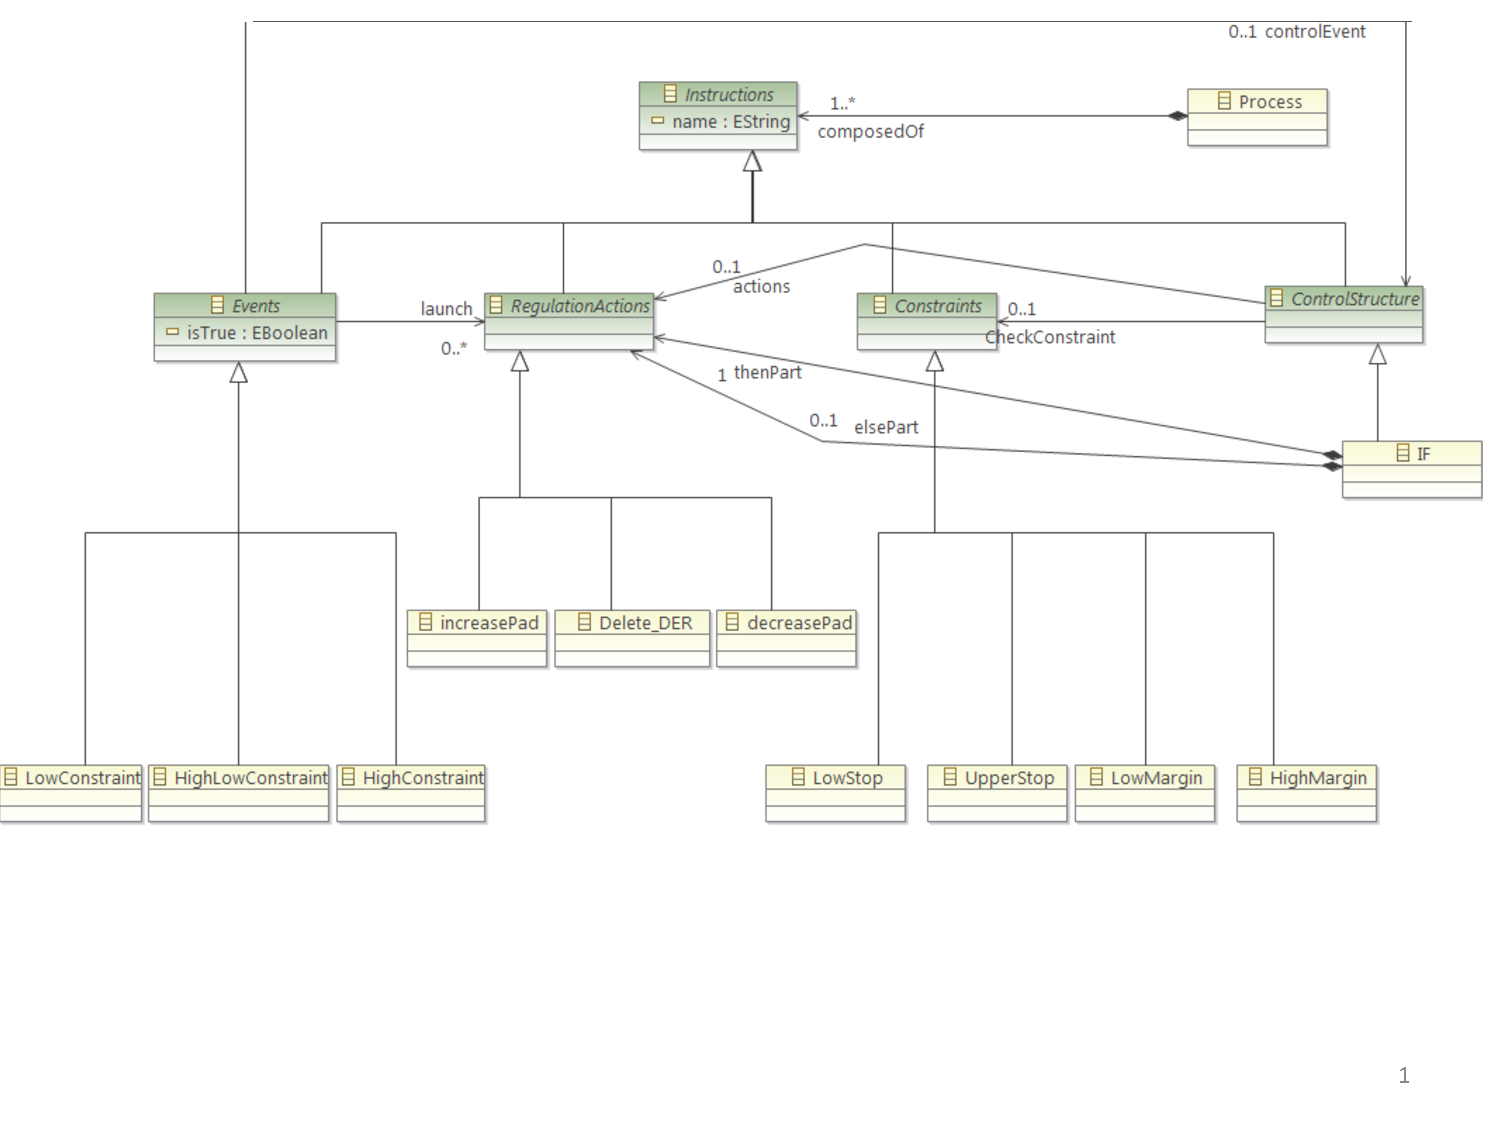
\includegraphics[trim = 0cm 5cm 0cm 0cm, clip, width=1\textwidth]{figures/6_methodologie/metamodele_dsml.pdf}
 \caption{Métamodèle d'un processus fonctionnel de régulation de tension \\
          sur un réseau de distribution électrique}
 \label{fig:meta_dsml}
\end{figure} 

Une syntaxe concrète et une sémantique d'exécution ont aussi été conçues pour ce
\gls{dsml}. Le DSML a ensuite été implémenté par un stagiaire dans
l'environnement Eclipse. L'utilisation d'Eclipse est largement répandue dans la
communauté de l'IDM. La fondation Eclipse héberge le projet \textit{Eclipse
Modeling} qui propose des langages et outils dédiées au développement de
\gls{dsml}. La sémantique d'exécution a été implémentée avec Kermeta. Kermeta
offre la possibilité de définir la sémantique d'exécution
directement au niveau du métamodèle à l'aide un langage d'action.


\subsection{Validation}
Le prototype ainsi implémenté permet de
créer et de simuler des processus fonctionnels pour la régulation de tension. La
figure~\ref{fig:proto_dsml} est une capture d'écran représentant le prototype. La
partie droite correspond à la palette de création de processus de régulation où
se trouvent les concepts du métamodèle sous leur forme graphique. La partie
gauche correspond à un exemple de processus modélisé avec cette palette.

\begin{figure}[!ht]
  \centering
  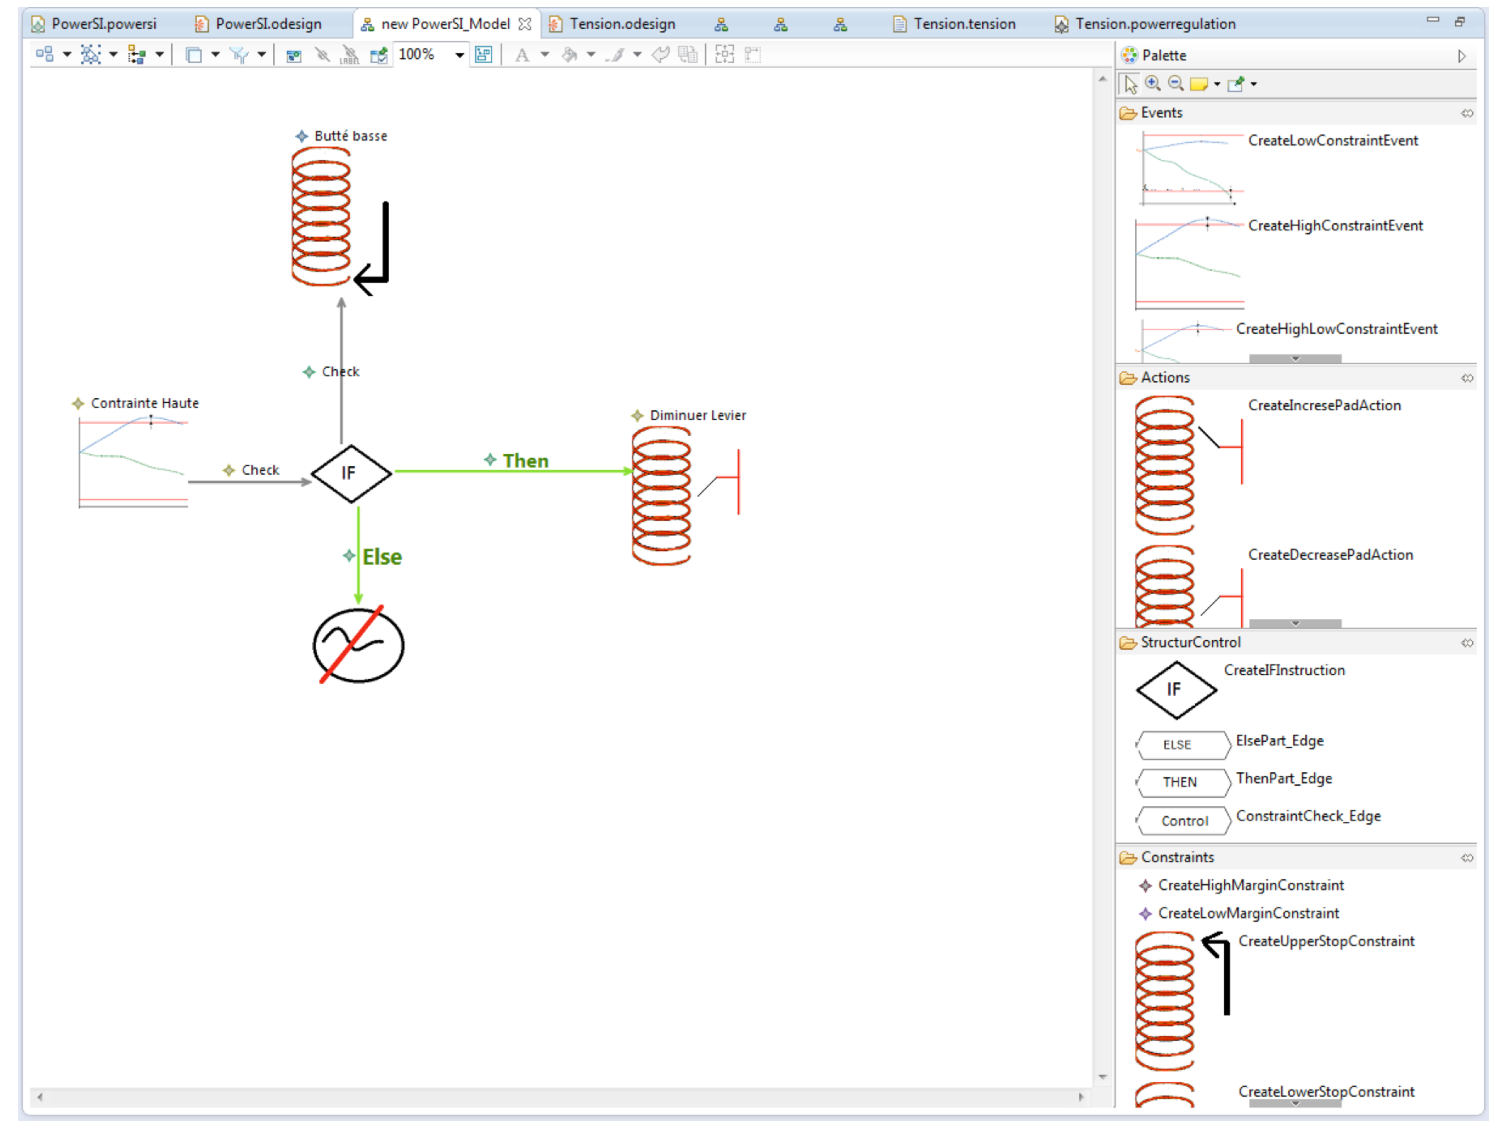
\includegraphics[trim = 0cm 0cm 0cm 0cm, clip, width=1\textwidth]{figures/6_methodologie/proto_dsml.pdf}
 \caption{Exemple de processus fonctionnel de régulation de tension modélisé avec le prototype de \gls{dsml}}
 \label{fig:proto_dsml}
\end{figure} 

Le prototype a été soumis à des personnes appartenant aux profils identifiés
dans l'observation, c'est-à-dire des personnes du domaine SI et des personnes du
domaine du réseau électrique. Les personnes du domaine SI sont principalement
des architectes SI. Leur retour a été positif. Ils ont trouvé dans le DSML
développé un moyen de modéliser des processus pour le métier et d'échanger avec
les personnes du domaine électrique qui ne maitrisent pas toujours les langages
traditionnellement utilisés dans le domaine SI comme UML. Le retour des
personnes du domaine du réseau électrique n'a pas été aussi enthousiaste que
celui des personnes du domaine SI. Il s'agit d'abord d'un problème de
sémantique. En effet, il n'ont pas vu d'intérêt à modéliser des « fonctions » de
conduite de réseau avec un nouveau DSML. Le terme « fonction » est associé au
domaine purement électrique et non SI. Or ces fonctions sont habituellement
modélisées avec les automates programmables ou encore le langage Matlab. Ces
langages sont éprouvés pour le domaine du réseau électrique mais ne sont pas
adaptés à la vue fonctionnelle du SI. Cette dernière ne met pas l'accent sur le
détail de l'implémentation de la fonction, mais plutôt sur l'orchestration des
différentes fonctions et leur structuration en blocs fonctionnels.

L'analyse du résultat des entretiens menés avec les personnes du domaine SI et
les personnes du domaine des réseaux électriques a validé partiellement les
hypothèses formulées à l'issue de l'observation. Ainsi, en montrant leur intérêt
pour le DSML, les personnes du domaine SI ont affirmé l'intérêt de modéliser et
de simuler le SI avec des langages compréhensibles par les personnes du métier,
en l'occurrence celles du domaine du réseau électrique.  En revanche, le retour
des personnes du domaine du réseau électrique a, au regard de notre analyse,
infirmé l'hypothèse selon laquelle la simulation des SI des Smart Grids est aussi
pertinente pour les SI industriels que pour les SI de gestion. En effet, les SI
industriels sont déjà l'objet de simulations (avec les automates programmables
et Matlab par exemple).

\subsection{Conclusion}
Cette dernière application du protocole
d'investigation à cette étude a permis en outre d'identifier deux types de SI
pour les Smart Grid. L'étude a confirmé la pertinence de la simulation de SI
pour la vue fonctionnelle, mais seulement pour un SI de gestion. Les SI purement
informatiques, autrement dit ceux qui ne font pas intervenir de tâche humaine et
qui pilotent directement les équipements électriques, ne sont pas concernés par
notre recherche. En effet, il existe déjà des langages dédiés à leur
modélisation et simulation (automates programmables et Matlab). Le terme «~SI
industriel~» employé pour qualifier ces systèmes a été, à notre sens, trompeur
dans le sens où il s'agit plutôt d'une restriction ou d'une spécialisation du
terme SI. En effet, selon la définition de Reix (cf. section~\ref{sec:reix}),
toute ressource intervenant sur le cycle de vie d'une information au sein d'une
organisation fait partie du SI, y compris le personnel.
	


\section{Conclusion}

Dans ce chapitre, nous avons abordé la question de la délimitation de l'objet d'étude.
Cette délimitation a été, en soi, à l'origine d'une démarche de recherche à part en entière.
Nous avons adopté une démarche inductive en définissant un protocole d'investigation que nous
avons appliqué à chacune des vues métier, fonctionnelle et applicative.
Nous avons ainsi pu jeter les bases des travaux précédemment présentés dans ce mémoire et 
mettre en évidence certaines caractéristiques de notre objet d'étude à savoir~:
(1)~la simulation du SI est pertinente pour valider/critiquer les scénarios des cas métier développés pour
les Smart Grids avant leur implémentation (2)~nos travaux seront plus pertinents pour les SI de
gestion que pour les SI industriels pour lesquels il existe déjà des méthodes et langages de simulation dédiés
(3)~la simulation est d'autant plus cruciale pour le SI, en le traitant dans sa globalité et en explicitant les interactions
entre ses macro-composants. 


		 


% 	\section{Conceptualisation / construction du cadre d'architecture 
% \textit{ExecuteEA}}
% %À partir de la compréhension empirique de notre objet d'étude et de la 
% formulation d'une problématique 
% La reformulation de la question de départ abouti à la définition d'une 
% problématique 
% La question de départ est au cœur de la problématique 

% permet la Définition du cadre théorique 

% La proposition est au contraire déductive
% Sujet identifiés, hypothèses formulées
% systèmes similaires : SI et entreprise -> établir les similarités
% Les hypothèses etc.  
% Choix de la théorie à appliquer : IDM (hypothèse et conclusion)/ apport de l'IDM 
% a-à l'EA, hypothèse (même problématique) à une échelle différente  ‹
% Itérative et là Smook 

% 	\subsubsection{Conclusion}
	

% L'observation menée à travers les entretiens et la revue des standards utilisés dans le domaine SI a permis d'identifier un nouveau langage de modélisation fUML. Encore en phase d'élaboration au sein de l'\gls{omg}, ce langage n'a pas pu être testé. Cependant, nous l'avons identifié comme candidat potentiel pour la simulation de diagrammes d'activité.

% Le protocole d'investigation s'est de plus révélé adéquat avec notre terrain d'étude. En effet, l

% Ces experts ne sont pas sensibilisés au domaine SI et considèrent les applications développées pour le réseau électrique comme partie intégrante de celui 

% Les investigations menées pour la vue applicative a permis de recentrer la simulation des les SI des Smart Grids sur la simulation de leurs SI uniquement sans traiter la question de la co-simulation SI/réseau électrique comme expliqué dans la section~\ref{sec:investig_appli}. 
	

